\documentclass{exerciseBlue}

\settitle[*le nice Summary]{Medical Robotics}
\addstudent[653897]{Alexander Osiik}
\usepackage{tikz}
\usepackage{pifont}
\usepackage{pgf}
\usepackage{graphicx}
\usepackage{listings}
\usetikzlibrary{positioning}
\usetikzlibrary{arrows,  automata, fit, shapes}
\usetikzlibrary{matrix}
\tikzstyle{mycircle }=[circle, draw, thick]
\tikzstyle{myrect }=[ circle ,draw ,thick]
\usepackage{pifont}% http://ctan.org/pkg/pifont
\newcommand{\cmark}{\ding{51}}%

\begin{document}
	\section{Applications of Medical Robotics}
	 There are 4 types of Robots
	  \begin{itemize}
	  	\item Robots for \textbf{Navigation}\ref{sec:navigation}\\
	  	\textit{Surgical drill} for Precise positioning, motion compensation..
	  	\item Robots for \textbf{Imaging}\\
	  	\textit{Minimally-invasive surgery} by Motion downscaling, reduce tremor...
		\item Robots for \textbf{Motion Replication}\\
		\textit{Robotic ultrasound} for Automation, speed...
		\item \textbf{Rehabilitation} and \textbf{Prosthetics}\\
		\textit{Exoskeletons} that Replace damaged structures, autonomous rehabilitation...
	  \end{itemize}
	  Application: Epiphyseolysis
  
  \section{Navigation}\label{sec:navigation}
  \subsection{Problem: We have an image.}
  \begin{itemize}
  	\item  Where is the \textbf{Robot} in the image coordinate system?
  	\item Where is the \textbf{Target} in the image?
  \end{itemize}  
\subsection{Ingridients for Radiologic Navigation:}
\begin{itemize}
	\item \textbf{C-Arm Robot:}\\
	A mobile x-ray system, robot containing 2 prismatic and 3 revolute Joints
	\item \textbf{Infrared Tracking:}\\
	Place Marker on Endeffector, on Target and on C-Arm. A Camera the ncalculates the positions:
	\begin{itemize}
		\item Skin incision
		\item Place marker on bone
		\item Take 2 C-Arm images
		\item Tavigate
	\end{itemize}
	\item[$\implies$] Navigation, Registration, Calibration!
\end{itemize}
\subsection{Spatial position and orientation}
Every Transformation is a multiplication, simply write down the vectors.\\
Rotatory Matrices:\\
$R(x,\theta) = \begin{pmatrix}
1&0&0&0\\
0&C_{\theta}&-S_{\theta}&0\\
0&S_{\theta}&C_{\theta}&0\\
0&0&0&1
\end{pmatrix}, \ 
R(y,\theta) = \begin{pmatrix}
C_{\theta}&0&S_{\theta}&0\\
0&1&0&0\\
-S_{\theta}&0&C_{\theta}&0\\
0&0&0&1
\end{pmatrix}, \ 
R(z,\theta) = \begin{pmatrix}
C_{\theta}&-S_{\theta}&0&0\\
S_{\theta}&C_{\theta}&0&0\\
0&0&1&0\\
0&0&0&1
\end{pmatrix}$\\
Translatory Matrices:\\
$T(x,a) = \begin{pmatrix}
1&0&0&a\\
0&1&0&0\\
0&0&1&0\\
0&0&0&1
\end{pmatrix}, \ 
T(y,a) = \begin{pmatrix}
1&0&0&0\\
0&1&0&a\\
0&0&1&0\\
0&0&0&1
\end{pmatrix}, \ 
T(z,a) = \begin{pmatrix}
1&0&0&0\\
0&1&0&0\\
0&0&1&a\\
0&0&0&1
\end{pmatrix}$
\subsection{Denavit Hartenberg Parameter}
TODO
\\
In \textbf{Forward Kinematics}, we derive the Endeffector Position by multiplication of given Joint Matrices, e.g.\\
$$^BM_G = ^BM_1 \cdot  ^1M_2 \cdot  ^2M_3 \cdot  ^3M_G$$
In \textbf{Reverse Kinematics}, we calculate the Joint angles from a given Endeffector Position, e.g. One Joint Robot:\\
$P = (P_X, P_Y), \ \text{Get Angle } \theta \text{ by:} \dfrac{P_Y}{P_X} = \dfrac{\sin \theta}{\cos \theta} = \tan \theta \implies \theta = atan2(P_Y, P_X)$\\
Use atan2-Function, as it gives back the angles of full circle depending on signs 
  \section{Navigation \& Registration}
  \subsection{Problem: We have >1 images.}
  \begin{itemize}
  	\item Rotate images in such way, that images align
  	\item Output is $\theta, \triangle x, \triangle y$
    \end{itemize}
There are various types of Registration:
\begin{itemize}
	\item point-based
	\item landmark-based
	\item contour-based
	\item intensity-based
	\item elastic
\end{itemize}
\subsection{Landmark based registration}
Situation: We have an MR image of a head. We place 4 Landmarks (Nose and Mouth). The Target Point is given with respect to the four landmark points. \\
From this, two point clouds $A,B$ are generated.\\
We assume: $\#A = \#B, \ 2D, \ a_1\rightarrow b_1 \ etc.$\\
If we move $B$, this leads to:\\\\
$b_1 \leadsto R\cdot b_1 + t$, $R = \begin{pmatrix}
	\cos \theta & -\sin\theta\\
	\sin\theta & \cos\theta
\end{pmatrix}, t = \begin{pmatrix}
t_x\\
t_y
\end{pmatrix}$\\
$b_2 \leadsto R\cdot b_2 + t$\\
$\vdots$\\
$b_n \leadsto R\cdot b_n + t$\\\\
We create a function $f$, which is the distance between the two point clouds $A$ and $B$. We want to minimize this function:
$$f = ||R\cdot b_1 + t - a_1||^2+\dots+||R\cdot b_n + t - a_n||^2$$
\subsection{Gaussian Least Square}
If we assume that the angle $\theta$ is small, we can linearize the rotational matrix R such that:
$$\cos \theta \sim 1, \ \sin \theta \sim \theta \implies R = \begin{pmatrix}
1 & -\theta\\
\theta & 1
\end{pmatrix}$$\\
This matrix $R$ is linear in $\theta$.\\
We can also linearize the 3D rotation matrix as follows:
$$R(x,\alpha)\cdot R(y,\beta)\cdot R(z,\gamma) = \begin{pmatrix}
1 & \gamma & -\beta\\
-\gamma & 1 & \alpha\\
\beta & \alpha & 1
\end{pmatrix}$$
As the multiplication of two small values leads to an even smaller value. This method works fine until angles of 10 degrees.
\subsection{Iterative Closest Points (ICP)}
 Assume we have a point cloud $A$ and a point cloud $ B$. We want know the transformation needed to overlap $B$ over $A$. We do \textbf{not} deform $B$, as all motion is rigid (rotation and translation).\\
 Cloud A: 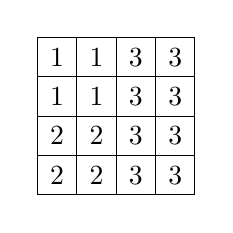
\begin{tikzpicture}
 \tikzset{square matrix/.style={
 		matrix of nodes,
 		column sep=-\pgflinewidth, row sep=-\pgflinewidth,
 		nodes={draw,
 			minimum height=#1,
 			anchor=center,
 			text width=#1,
 			align=center,
 			inner sep=0pt
 		},
 	},
 	square matrix/.default=.5cm
 }
 %|[fill=yellow]|
 \matrix[square matrix]
 {
 	1 & 1 & 3 & 3 \\
 	1 & 1 & 3 & 3 \\
 	2 & 2 & 3 & 3 \\
 	2 & 2 & 3 & 3 \\
 }; 
 \end{tikzpicture}
 Cloud B
  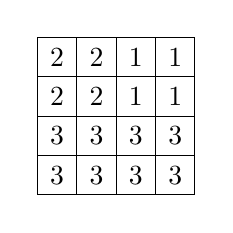
\begin{tikzpicture}
 
 \tikzset{square matrix/.style={
 		matrix of nodes,
 		column sep=-\pgflinewidth, row sep=-\pgflinewidth,
 		nodes={draw,
 			minimum height=#1,
 			anchor=center,
 			text width=#1,
 			align=center,
 			inner sep=0pt
 		},
 	},
 	square matrix/.default=.5cm
 }
 %|[fill=yellow]|
 \matrix[square matrix]
 {
 	2 & 2 & 1 & 1 \\
 	2 & 2 & 1 & 1 \\
 	3 & 3 & 3 & 3 \\
 	3 & 3 & 3 & 3 \\
 }; 
 \end{tikzpicture}
 $\implies $ Just rotate $90^o$ to align\\
 But sometimes, coloring differs in images depending on the imaging process. For Example, in CT the bone has a bright white color, while in MR the bone is more gray:\\
  Cloud A: 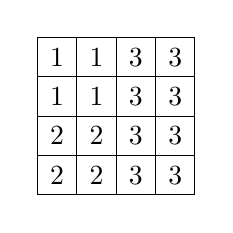
\begin{tikzpicture}
 \tikzset{square matrix/.style={
 		matrix of nodes,
 		column sep=-\pgflinewidth, row sep=-\pgflinewidth,
 		nodes={draw,
 			minimum height=#1,
 			anchor=center,
 			text width=#1,
 			align=center,
 			inner sep=0pt
 		},
 	},
 	square matrix/.default=.5cm
 }
 %|[fill=yellow]|
 \matrix[square matrix]
 {
 	1 & 1 & 3 & 3 \\
 	1 & 1 & 3 & 3 \\
 	2 & 2 & 3 & 3 \\
 	2 & 2 & 3 & 3 \\
 }; 
 \end{tikzpicture}
 Cloud B
 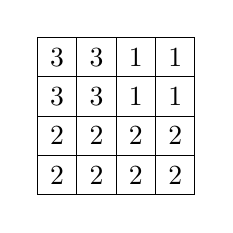
\begin{tikzpicture}
 
 \tikzset{square matrix/.style={
 		matrix of nodes,
 		column sep=-\pgflinewidth, row sep=-\pgflinewidth,
 		nodes={draw,
 			minimum height=#1,
 			anchor=center,
 			text width=#1,
 			align=center,
 			inner sep=0pt
 		},
 	},
 	square matrix/.default=.5cm
 }
 %|[fill=yellow]|
 \matrix[square matrix]
 {
 	3 & 3 & 1 & 1 \\
 	3 & 3 & 1 & 1 \\
 	2 & 2 & 2 & 2 \\
 	2 & 2 & 2 & 2 \\
 }; 
 \end{tikzpicture}
 $\implies $ rotate $90^o$ enough?\\
\subsection{Mutual Information (MI)}
For \textbf{Mutual Information} Registration, the color mapping does not have to be exactly 1x1. It can be different, as shown in the example above.\\
\textbf{Basic Definition:}\\
We generate Images $A,B$ in a random process. For each pixel of the image, we throw a dice (random generation), so we map 6 colors $\{1,\dots,6\}$ to each pixel. $A,B$ are random variables with distributions $P_A, P_B$, namely:
\begin{itemize}
	\item $P_A(a) = $ Probability of grey level value $a$ in image $A$ 
	\item $P_B(b) = $ Probability of grey level value $b$ in image $B$
	\item[$\implies$] $P_{A,B}(a,b) = $ Probability of grey level value $a$ in image $A$ occuring at the same position in image $B$ 
\end{itemize} 
Examples:
\begin{itemize}
	\item $A \neq B:$ $A$ tells nothing about $B$, 2 different images
	\item $A = B: $ $A$ tells everything about $B$ 
	\item $A$ tells something about $B$
\end{itemize}
Keep in mind the law of Independence of two random variables:
$$P_{A,B}(a,b) = P_A(a)\cdot P_B(b)$$
We want to know the maximum Mutual Information, calculated as follows:\\
$$I(A,B) = \sum_{a,b}P_{A,B}(a,b)\cdot \log_2 \left(\dfrac{P_{A,B}(a,b)}{P_A(a)\cdot P_B(b)}\right)$$
The Sum ranges over all greyscale pairs of diefferent colors. $I(A,B)$ measures the information dependencies. We maximize the Mutual Information to find exact position.\\
Example 1:$$A = 
 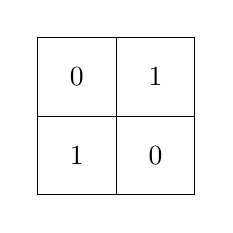
\begin{tikzpicture}

\tikzset{square matrix/.style={
		matrix of nodes,
		column sep=-\pgflinewidth, row sep=-\pgflinewidth,
		nodes={draw,
			minimum height=#1,
			anchor=center,
			text width=#1,
			align=center,
			inner sep=0pt
		},
	},
	square matrix/.default=1cm
}
%|[fill=yellow]|
\matrix[square matrix]
{
	0 & 1 \\
	1 & 0  \\
}; 
\end{tikzpicture}, \ \ B = 
 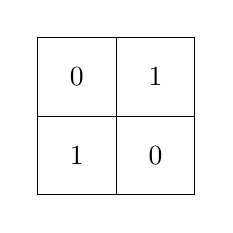
\begin{tikzpicture}

\tikzset{square matrix/.style={
		matrix of nodes,
		column sep=-\pgflinewidth, row sep=-\pgflinewidth,
		nodes={draw,
			minimum height=#1,
			anchor=center,
			text width=#1,
			align=center,
			inner sep=0pt
		},
	},
	square matrix/.default=1cm
}
%|[fill=yellow]|
\matrix[square matrix]
{
	0 & 1 \\
	1 & 0  \\
}; 
\end{tikzpicture}$$
$$P_A(0) = 0.5, \ P_B(0) = 0.5$$
$$P_A(1) = 0.5, \ P_B(1) = 0.5$$
$$P_{A,B}(0,0) = 0.5, \ P_{A,B}(0,1) = 0$$
$$P_{A,B}(1,1) = 0.5, \ P_{A,B}(1,0) = 0$$
$$\sum = 1$$
$$I(A,B) = \sum_{a,b}P_{A,B}(a,b)\cdot \log_2 \left(\dfrac{P_{A,B}(a,b)}{P_A(a)\cdot P_B(b)}\right)$$
$$= 0.5 \cdot \log_2 \left(\dfrac{P_{A,B}(0,0)}{P_A(0)\cdot P_B(0)}\right) + 0.5\cdot \log_2 \left(\dfrac{P_{A,B}(1,1)}{P_A(1)\cdot P_B(1)}\right) + 0\cdot \log_2 \left(\dfrac{P_{A,B}(0,1)}{P_A(0)\cdot P_B(1)}\right) + 0\cdot \log_2 \left(\dfrac{P_{A,B}(1,0)}{P_A(1)\cdot P_B(0)}\right)$$
$$= 0.5 \cdot \log_2 (2) + 0.5 \cdot \log_2(2)$$
$$= 1$$
Example 2:$$A = 
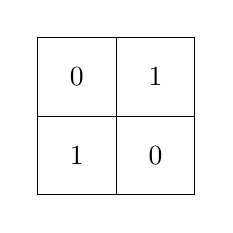
\begin{tikzpicture}

\tikzset{square matrix/.style={
		matrix of nodes,
		column sep=-\pgflinewidth, row sep=-\pgflinewidth,
		nodes={draw,
			minimum height=#1,
			anchor=center,
			text width=#1,
			align=center,
			inner sep=0pt
		},
	},
	square matrix/.default=1cm
}
%|[fill=yellow]|
\matrix[square matrix]
{
	0 & 1 \\
	1 & 0  \\
}; 
\end{tikzpicture}, \ \ B = 
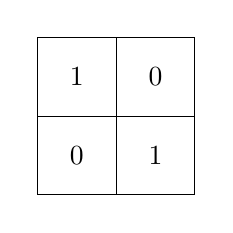
\begin{tikzpicture}

\tikzset{square matrix/.style={
		matrix of nodes,
		column sep=-\pgflinewidth, row sep=-\pgflinewidth,
		nodes={draw,
			minimum height=#1,
			anchor=center,
			text width=#1,
			align=center,
			inner sep=0pt
		},
	},
	square matrix/.default=1cm
}
%|[fill=yellow]|
\matrix[square matrix]
{
	1 & 0 \\
	0 & 1  \\
}; 
\end{tikzpicture}$$
$MI(A,B) = 1$, as we care for the structure of the image. The color values do not really matter.
Example 3:$$A = 
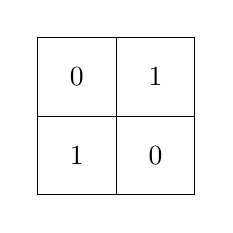
\begin{tikzpicture}

\tikzset{square matrix/.style={
		matrix of nodes,
		column sep=-\pgflinewidth, row sep=-\pgflinewidth,
		nodes={draw,
			minimum height=#1,
			anchor=center,
			text width=#1,
			align=center,
			inner sep=0pt
		},
	},
	square matrix/.default=1cm
}
%|[fill=yellow]|
\matrix[square matrix]
{
	0 & 1 \\
	1 & 0  \\
}; 
\end{tikzpicture}, \ \ B = 
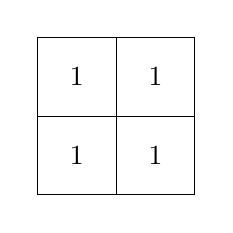
\begin{tikzpicture}

\tikzset{square matrix/.style={
		matrix of nodes,
		column sep=-\pgflinewidth, row sep=-\pgflinewidth,
		nodes={draw,
			minimum height=#1,
			anchor=center,
			text width=#1,
			align=center,
			inner sep=0pt
		},
	},
	square matrix/.default=1cm
}
%|[fill=yellow]|
\matrix[square matrix]
{
	1 & 1 \\
	1 & 1  \\
}; 
\end{tikzpicture}$$
$MI(A,B) = 0$, as the structures are very different.
Example 4:$$A = 
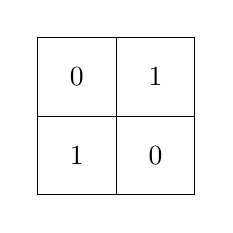
\begin{tikzpicture}

\tikzset{square matrix/.style={
		matrix of nodes,
		column sep=-\pgflinewidth, row sep=-\pgflinewidth,
		nodes={draw,
			minimum height=#1,
			anchor=center,
			text width=#1,
			align=center,
			inner sep=0pt
		},
	},
	square matrix/.default=1cm
}
%|[fill=yellow]|
\matrix[square matrix]
{
	0 & 1 \\
	1 & 0  \\
}; 
\end{tikzpicture}, \ \ B = 
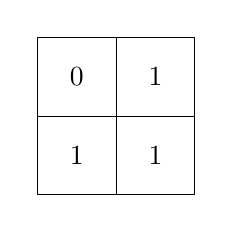
\begin{tikzpicture}

\tikzset{square matrix/.style={
		matrix of nodes,
		column sep=-\pgflinewidth, row sep=-\pgflinewidth,
		nodes={draw,
			minimum height=#1,
			anchor=center,
			text width=#1,
			align=center,
			inner sep=0pt
		},
	},
	square matrix/.default=1cm
}
%|[fill=yellow]|
\matrix[square matrix]
{
	0 & 1 \\
	1 & 1  \\
}; 
\end{tikzpicture}$$
$MI(A,B) = 0.32$\\
Keep in mind that $MI\geq0$, but can go up to 100 for large images!
\subsection{Calculating $P_A$, $P_B$, $P_{A,B}$}
Just create a table, then divide the right hand side by the amount of pixels/voxels:\\
$$\begin{tabular}{l|l}
	\hline
	0 & number of Pixels in image $A$ with greylevel 0\\
	$\vdots$ & $\vdots$\\
	255 & number of Pixels in image $A$ with greylevel 255\\
\end{tabular}$$\\
Calculating $P_{A,B}$ is a little difficult:\\
$$\begin{tabular}{l|lll}
	& 0 $\dots$ & $i$ & $\dots$ 255\\
	\hline
	0 & & & \\ 
	$\vdots$ & & \vdots &\\
	$i$ & \dots &\# pixel pins with colors $i,j$ &\\
	$\vdots$ & & &\\
	255 & & & \\
\end{tabular}$$
There are 3 algorithms/methods for calculation:
\begin{itemize}
	\item[1.] \textbf{Nearest Neighbour (NN)}
	\item[2.] \textbf{Trilinear Interpolation (TI)}
	\item[3.] \textbf{Trilinear Partial Volume (TPV)}
\end{itemize}
  \section{Imaging}\label{sec:imaging}
  \subsection{Image Deformation}
  There are multiple applications:
  \begin{itemize}
  	\item Elastic Registration 
  	\item Distortion Correction
  \end{itemize}
\subsubsection{Bilinear Onterpolation}
Assume we have 2 adjacent grid points $u,v$. To get from $G'$ to $G$ we have to deform $u$ in x-direction by $du$. We obtain information for $w$ by \textbf{linear interpolation}. Same for the y-direction.\\
\textbf{Advantage:} \begin{itemize}
	\item Simplicity
	\item We will move all points to its goal $\implies$ Accuracy!
\end{itemize}
\textbf{Disadvantage:} \begin{itemize}
	\item Not smooth
\end{itemize}
\subsubsection{Cubic Spline Interpolation}
We define a correction polynomial, two variables $x,y$
$$a_0 + a_1x+a_2y+a_3xy+a_4x^2+a_5y^2+a_6xy^2+a_7x^2y+a_8x^3 + a_9y^3$$
$$b_0 + b_1x+b_2y+b_3xy+b_4x^2+b_5y^2+b_6xy^2+b_7x^2y+b_8x^3 + b_9y^3$$
We have our model: $(x_m,y_m)$ and our distorted points $(x_d,y_d)$.\\
We further assume, that $a$'s and $b$'s are variables, while $x,y$ are constant.\\
We set up $f$ as:
$$f = [(x_m,y_m)-(x_d,y_d)]^2$$
For $N$ grid points, we adjust $f$ to:
$$f = [(x_m^{(1)},y_m^{(1)})-(x_d^{(1)},y_d^{(1)})]^2 + \dots + [(x_m^{(N)},y_m^{(N)})-(x_d^{(N)},y_d^{(N)})]^2$$
With $x_d$ being the $a$-Polynomial and $x_m$ being the $b$-Polynomial, function $f$ is quadratic in the $a$'s and $b$'s.\\
We deriviate $f$ after $a_i,b_i$, with:\\
$$\dfrac{\delta f}{\delta a_i} =\dfrac{\delta f}{\delta b_i} = 0$$
This is a 20x20 linear system. We perform Gaussian Elimination\\ $\implies$ \textbf{Gaussian Least Squares}\\
\textbf{Advantage:} \begin{itemize}
	\item Deformation will be smooth
\end{itemize}
\textbf{Disadvantage:} \begin{itemize}
	\item We can only create $\sim$-formed Formations. This prevents overfitting, but, regarding grid points, they will not always match.
\end{itemize}
\subsubsection{Thin Plate splines}
We describe deformation not only as a force on a specific point, but as da force on some entire sheet. So, we have $N$ points $p_1, \dots , p_N$ and we have a vector $z_1,\dots, z_N$ for each point. We set up function $f$ to represent deformation:
$$f(p) = \sum_{i=1}^{N} w_iF(||p-p_i||)$$
where $w_i$ are the weights and $F$ is our \textbf{Kernel function} 
$$F(r) = r^2 \ \ \ \text{or} \ \ \ F(r)=r^2\log r$$
\newpage\textbf{How to find the weight values?}\\
We have $N$ equations
$$f(p_1) = \sum_{i=1}^{N} w_iF(||p_1-p_i||) = z_1$$
$$\vdots$$
$$f(p_N) = \sum_{i=1}^{N} w_iF(||p_N-p_i||) = z_N$$
Our method of choice is to add 3 more equations to obtain a full linear system:
$$f(p) = \sum_{i=1}^{N} w_iF(||p-p_i||) + a_0 + a_1\cdot x + a_2\cdot y$$
where
$$\sum_{i=1}^{N}w_i = \sum_{i=1}^{N}x_i\cdot w_i = \sum_{i=1}^{N}y_i\cdot w_i = 0$$
\subsection{Elastic Registration}
Problem: We have to find correspondencies between landmarks.\\
We select/take a small subwindow on (e.g. $9\times9$ Pixel Array), and find the best match. We can find good landmarks by the use of \textbf{color contrasting} and \textbf{bimodal histograms.} We then use the histograms to replace elastic registration by correlation and prediction.
\subsubsection{Hand-Eye-Calibration}
We have a Robot. We know the Robots Forward Kinematics from base to endeffector (see. DH-Parameters or Handbook).\\
We place a marker on the bone/target and a marker on the endeffector. We observe via a camera.
$$\underbrace{^RT_E}_{known}\cdot \underbrace{^ET_M}_{unknown} = \underbrace{^RT_C}_{unknown} \cdot \underbrace{^CT_M}_{known}$$
$$\leadsto A\cdot x = y \cdot B$$
We have $24$ unknown variables, but only $12$ equations. What shall we do?\\
The trick is to move the robot, sinse $x,y$ are constant and won't change at all!
$$A_1 \cdot x=y \cdot B_1$$
$$A_2 \cdot x=y \cdot B_2$$
$$\vdots$$
$$A_{500} \cdot x=y \cdot B_{500}$$
\section{Treatment Planning}
\textbf{Situation:} We perform a surgery without CT (very slow), only X-Ray. We want to fix a bone, see picture. This is a heavily invasive operation, as we have to place implants to hold together the pieces. \\
To place an implant, we need to dril a hole into a bone to create a cavity for the implant. We drill before we cut the bone $\implies$ Cunjuction with Navigation. We have to drill at a correct angle, otherwise a (ugly) correction with screws is needed. As we are in 3D space, we don't have only one but \textbf{three} angles.\\
\textbf{Steps:}
\begin{enumerate}
	\item[1.] Take two x-ray images
	\item[2.] Extract relevant ``features'' of the geometry
	\item[3.] Plan (compute wedge planes)
	\item[4.] Navigate
\end{enumerate}
\noindent\rule{\textwidth}{0.3pt}
\begin{enumerate}
	\item[1.] \cmark (AP and lateral x-ray)
	\item[2.] \begin{itemize}
		\item femur shaft axis
		\item femur neck isthmus
		\item femur head center point
		\item cutting plane
	\end{itemize}
	\textbf{Steps for feature extraction (point)}
	\begin{itemize}
		\item mark point in x-ray in both images. The C-Arm has amarker, the positions are known
		\item Get the line
		\item Intersect two lines
		\item Define the base coordinate system
		\item Origin is defined as the intersection of shaft axis and cutting plane
		\item z-axis points along the shaft axis
		\item y-axis: AP in images
		\item x-axis: Put in such way that the right hand coordinate system is complete
	\end{itemize}
	\item[3.] Plan (compute wedge planes)
	\item[4.] Navigate
\end{enumerate}
For the Computer Simulation, we define 3 angles:
\begin{itemize}
	\item flexion angle (x-axis)
	\item valgus angle (y-axis)
	\item rotation (z-axis)
\end{itemize}
\subsection{Planning for radiosurgery}
\textbf{Scenario:} We perform radiosurgery, which means we shoot beams to destroy a specific target in a human body. In order not to damage the surrounding tissue unnecessarily, we shoot various low power beams from various directions, instead of a high power beam from one. By this, we have a high dose in the target and a low intensity in the tissue. The robot performs ``Step-And-Shoot''.\\
\textbf{Problems:}
\begin{itemize}
	\item Radiation is physical, it spreads
	\item If we go around some important object, we will have an overdose on the inner track and an underdose on the outer track
	\item How long do we have to activate a beam at which position?\\
	$\implies$ We have to place \textbf{beams} and calculate the \textbf{weights}.
\end{itemize}
\subsubsection{Specification of Goals}
\begin{itemize}
	\item[1.] We want to achieve dose homogenity. It has to be homogenious in the tumor
	\item[2.] We want to protect the critical region / minimal dose threshold. We specify a minimum value in tumor and a maximum value in tissue.
	\item[3.] We want to have a high dose gradient around the target
	\item[4.] Conformity
\end{itemize}
To achieve this, we have to \textbf{deliniate the target} on each positive CT slice, \textbf{deliniate the critical region} and \textbf{enter the values} as (upper/lower) threshold.
\subsubsection{Beam Weights Computation (LP)}
We have multiple equations, the $a$'s and $b$'s are either 0 or 1 (Beam Active or Not):

$$a_{1,1}x_1 + \dots + a_{1,n}x_n \leq critical_1$$
$$\vdots$$
$$a_{m,1}x_1 + \dots + a_{m,n}x_n \leq c_m$$
\noindent\rule{\textwidth}{0.3pt}
$$b_{1,1}x_1 + \dots + b_{1,n}x_n \leq tumor_1$$
$$\vdots$$
$$b_{m,1}x_1 + \dots + b_{m,n}x_n \leq t_m$$
We call this the \textbf{Linear Feasability Problem (F)}
\subsubsection{General Linear Programming}
Minimize
$$\min c_1x_1 + \dots c_nx_n$$
Such that all $m$ constraints are met
$$a_{1,1}x_1 + \dots + a_{1,n}x_n \leq b_1$$
$$\vdots$$
$$a_{m,1}x_1 + \dots + a_{m,n}x_n \leq b_m$$
\textbf{Implicit constraint:} $x_i \geq 0$, beams can not be negative.
\par
(F) and (LP) are very similar. In fact, (LP) is just (F) with additional minimization or maximization function. Each constraint specifiec one line, alltogether they specify the solvable region containing feasable point, as they satisfy the equation.\\
Linear Programming is the origin for \textbf{Support Vector Machines}. How do we solve (LP)?\\
Each constraint gives us 1 line. (LP) always returns a vertex of the feasable region.
\par The \textbf{Naive Method for LP} is to look at linear equation systems, and to look at all $n$-pels (pairs of $n$ constraints) from all $m+n$ constraints. The solutions are, as always, the intersection points.
\subsubsection{Infeasibility}
How do we deal with infeasibility? Well, we take the original constraint
$$a_{1,1}x_1 + \dots + a_{1,n}x_n \leq b_1$$
and modify it by inserting 2 new variables $s_1,s_1'$
$$a_{1,1}x_1 + \dots + a_{1,n}x_n+s_1-s_1' \leq b_1$$
Now, we want to minimize the deviation from the original constraint:\\
$$\min s_1+\dots + s_m + s_1' + \dots + s_m'$$
\subsubsection{Hierarchy of shapes}
The most simple shape is a sphere. The \textbf{Isocenter} is in the center of the sphere.\\
Next would be an ellipse. The problem is, that an ellipse fits 2 spheres (and two isocenters), but not the whole area is covered, creating hot spots (area covered multiple times) and cold spots (area not covered at all). The solution is to sweep through the area, and the cold spots will vanish.\\
The area of a tumor will get smaller, if we put isocenters around the tumor (on it's surface) and erase the covered area.\\
\textbf{Problems:} \begin{itemize}
	\item The dose decreases with depth in tissue
	\item There is an off center ratio
\end{itemize} 
\subsection{Overall Planning}
\begin{enumerate}
	\item[1.] Deliniate target (polygon), set dose thresholds (initial and target)
	\item[2.] Inverse Planning \begin{itemize}
		\item Beam Placement
		\item Beam Weights
	\end{itemize}
\item[3.] Forward dose and visualize
\end{enumerate}
\section{Motion Correlation and Tracking}
Most of the time, we have to use some sort of 4D Planning, because the target moves (e.g. patient breathes). To track a moving target with a robot, we need special sort of imaging that is fast enough to calculate.\\
CT and MR are too slow for tracking. So, we create a model that predicts certain motion patterns. We claim that the motions correlate, as they tend to be similar over time.\\
Thus, the general idea is to \textbf{infer the target position} (which we don't see) from skin motion (which we see). We place IR Markers on the skin and gold markers near the tumor to perceive the movement. We then get the real position every timestep $T_i$, create the correlation, and predict the positions between $T_i$ and $T_{i+1}$. Summing up, we capture the \textbf{Motion Correlation} between skin motion and tumor and, by correlation, we then imply the target's position. \\
\subsection{Mathematics behind it: Computing Correlation}
In the set of data points, we want to find a regression line that fits to the data. To find the correlation, we use the \textbf{Gaussian Least Squares Method}.\\
For every data point, we have the $x$ and $y$ coordinates. Now, we have to find the $m$ (slope) and the $b$ (offset). we do so by minimizing the function $f$:
$$f = (y_1-mx_1-b)^2+(y_2-mx_2-b)^2+(y_3-mx_3-b)^2+\dots$$
\textbf{Problem:} Hysteresis (variant delayed behaviour of the caused output variable)\\
Reality is very noisy, and perceived motions are curves, not lines.\\
\textbf{Solution: Machine Learning}
We use support vector machines, as they are flexible and suitable for heterogeneous data.
\subsection{Motion Prediction}
We do get the real time position of the target, but the information is always delayed. We have to compensate for the time lag of robot movement, as the robot is always behind/latent.\\
We prepare training data set with equidistant spacing between the data points. By this, the information is evenly spaced, but the SVM does not know that. Also, we have to tell the SVM that the most recent calculated point is the most important one.
\subsection{MULIN: Multi-step Linear Interpolation}
$p(n)$: patient in time step $n$\\
$r(n)$: robot in time step $n$\\
$\implies $ To predict $p$ means to compute $p(n+1)$!\\
\par We define
$$p(n+1) = p(n) + [\underbrace{p(n)-r(n)}_{\text{Error in last step}}]$$
By this, error $e$ should be easier to predict than $p$, as $e$ has a way smaller amplitude than $p$:\\\\
$r(n) = p(n-1)$\\
$p(n+1) = p(n) + [\underbrace{p(n)-p(n-1)}_{e(n)}]$\\
$e(n+1) = e(n)+[e(n)-e(n-1)] = e^*$, this is MULIN of order 1\\
$p(n+1)=p(n)+e(n+1)$\\
Now, our goal is to predict $e^*$:
$$e^*(n+1) = e^*(n)+[e^*(n)-e^*(n-1)]$$
How far do we look into the past?
\subsubsection{Fast Lane Method}
We select a parameter $k$ which is the best/fastest. We keep $k$ until some other $k'$ becomes best. (Switch lanes like on ze gud old Autobahn).
\subsection{LMS Prediction}
We see that Robot Control has a lot to do with learning.\\
$e_{n+1} = y_{n+1} - y_{n+1}^{\text{LMS}}$\\
$y_{n+1}^{\text{LMS}} = w_n \cdot y_n$, where $w_n$ is the weight factor
$w_{n+1} = w_n + \mu \cdot e_n\cdot y_n$\\
\noindent\rule{\textwidth}{0.3pt}
$w_0 = 1$\\
$y_0^{\text{LMS}} = y_0$\\
$\mu = 2$
$E_{n+1} = (y_{n+1} - y_{n+1}^{\text{LMS}})^2$\\
$\frac{\delta E_{n+1}}{\delta w} = ?$\\
\noindent\rule{\textwidth}{0.3pt}
$E_{n+1} = (y_{n+1} - w_n\cdot y_n)^2$ per definition of $y_{n+1}^{\text{LMS}}$\\
$\dfrac{\delta E_{n+1}}{\delta w} = 2(y_{n+1}-w_n\cdot y_n)\cdot (-y_n)$\\
$ = 2(\underbrace{y_{n+1}-y_{n+1}^{\text{LMS}}}_{e_{n+1}})\cdot (-y_n)$\\
$ = 2\cdot e_{n+1}\cdot (-y_n) = -2\cdot e_{n+1}\cdot y_n$
\par aAssume error in last step is equal to this step. We then replace $e$ by $e_{n+1}$. To reduce the error, we must reduce $w$. Vice Versa, if the Gradient is negative, we must increase $w$:
\begin{itemize}
	\item[$\implies$] If Gradient \textbf{pos}, reduce $w$ to reduce $E$
	\item[$\implies$] If Gradient \textbf{neg}, increase $w$ to reduce $E$
\end{itemize}
\textbf{In comparision with MULIN, LMS is not as robust.}
 
\section{Motion Replication}\label{sec:motion}
Motion Replication is basically a scenarion of two robots, where the \textbf{replicator} imitates the motion of the \textbf{master}. This is a popular choice for\\\begin{itemize}
	\item Microsurgery
	\item Motion scaling for deliquate operations
	\item Tremor filtering
\end{itemize}
We want to conclude from the past, what is what and which is which. Most of the time, Robots are not position oriented, but rather force oriented (You usually calculate Current$\rightarrow$Force$\rightarrow$Angle$\rightarrow$Position)\\
\textbf{Problems:}\begin{itemize}
	\item We have to compensate gravity (which is also different in different parts on the planet!)
	\item We have to compensate lag (unwanted Overreaction)
\end{itemize}
For data acquisition, we can use:
\begin{itemize}
	\item[(i)] Force Sensors in every joint of the robot
	\item[(ii)] Torque Sensors in every joint
	\item[(iii)] Redundant Force measurements by combination of (i) and (ii)
	\item[(iv)] Cables. This is a popular choice as they compensate lag and the friction bounds gravity effects, see daVinci Robot
\end{itemize}
Assume a force $f$ acts on position $r$. We can calculate vector $\vec{t}$ by building the cross product of $\vec{r}$ and $\vec{f}$. Vector $\vec{t}$ is then orthogonal to the $\vec{r}$ and $\vec{f}$, and it's magnitude is the torque $\tau$: 
$$\vec{t} = \vec{r} \times \vec{f}$$
$$\tau = ||\vec{t}||, \ \ \text{unit Nm}$$
\noindent\rule{\textwidth}{0.3pt}
Calculation:
$r_1 = \begin{pmatrix}
l_1\cdot \cos_{\theta_1}\\l_1\cdot\sin_{\theta_1}\\0
\end{pmatrix} \implies \text{ For further } r_i \text{just add the lengths and angles}$
$\vec{t_n} = \vec{r_n} \times \vec{f}, \ \ \ \vec{t_{n-1}} = (\vec{r_n} + \vec{r_{n-1}}) \times \vec{f}$ and so on
\subsection{General Case (3D Robot, n joints)}
We want to transfor $\vec{f}$ to effector coordinate system.\\
For an $n$-Joint robot, the torques are calculated through
$$\begin{pmatrix}
\tau_1\\\vdots\\\tau_n
\end{pmatrix} = \begin{pmatrix}
z_0 \times (p_n - p_0)\\\vdots\\ z_{n-1} \times (p_n - p_{n-1})
\end{pmatrix}\cdot ^\textbf{B}f$$
where the matrix is the \textbf{Geometric Jacobian of the Robot}
\subsection{Robot Dynamics: A thought experiment}
Assume we have a person sitting in a chair. We have to possibilities to get up:
\begin{itemize}
	\item get up slowly: We need a counter weight (lean more forward)
	\item get up fast: We use our inertia
\end{itemize} 
Interestingly, the paths from both approaches are different.\\
\par In \textbf{Robot Dynamics}, we use the equation of motion, velocity and acceleration as funtion of position:\\\\
$\theta(t)$ is the joint \textbf{angle} as function of time\\
$\dot{\theta} = \theta'(t)$ is the \textbf{velocity} of the joint\\
$\ddot{\theta} = \theta''(t)$ is the \textbf{acceleration} in the joint\\\\
We further recall the \textbf{Kinetic Energy} $\mathcal{K}$ as
$$\mathcal{K} = \dfrac{1}{2}\cdot m \cdot v^2$$ and the \textbf{Potential Energy} $\mathcal{P}$ as
$$\mathcal{P} = m\cdot g \cdot h$$
\noindent\rule{\textwidth}{0.3pt}
The position $r(t)$ is calculated by (assume only x and y axis as in figure)
$$r(t)=\begin{pmatrix}
l\cdot \sin (\theta)\\0\\-l\cdot \cos (\theta)
\end{pmatrix}, \ \dot{r}=\begin{pmatrix}
l\cdot \cos (\theta) \cdot \dot{\theta}\\0\\l\cdot \sin (\theta)\cdot \dot{\theta}
\end{pmatrix}$$
$$\mathcal{K} =  \dfrac{1}{2}\cdot m \cdot (\dot{r})^2$$
$$=\dfrac{1}{2}\cdot m\cdot l^2 \cdot \dot{\theta}^2 \cdot [\underbrace{\cos^2(\theta)+\sin^2(\theta)}_{=1}]=\dfrac{1}{2}\cdot m\cdot l^2 \cdot \dot{\theta}^2$$
$$\mathcal{P} = m\cdot g \cdot h$$
$$=-m\cdot g \cdot l\cdot\cos (\theta)$$
\subsection{Lagrange Theorem}
We define the Lagragne Function with independent parameters $\theta,\dot{\theta}$
$$L(\theta,\dot{\theta}) = \mathcal{K}(\theta, \dot{\theta})-\mathcal{P}(\theta)$$
We then calculate the torque magnitude $\tau$ through Lagrange Theorem
$$\dfrac{d}{dt}\dfrac{\delta L}{\delta \dot{\theta}}-\dfrac{\delta L}{\delta \theta} = \tau$$
Note that $dt$ is a 1D differentiation, and $\delta \dot{\theta}$ is a partial differentiation.\\
Continuing:
$$L = \dfrac{1}{2}\cdot m \cdot l^2 \cdot \dot{\theta}^2 + m\cdot g \cdot l\cdot\cos (\theta)$$
$$\dfrac{\delta L}{\delta \dot{\theta}} = m \cdot l^2 \cdot \dot{\theta}$$
$$\dfrac{d}{dt}\dfrac{\delta L}{\delta \dot{\theta}} = m \cdot l^2 \cdot \dot{\theta} $$
$$\dfrac{\delta L}{\delta {\theta}} = -m\cdot g \cdot l\cdot\sin (\theta)$$
In conclusion, our torque is 
$$\tau = m \cdot l^2 \cdot \dot{\theta} + m\cdot g \cdot l\cdot\sin (\theta)$$
We see that the Lagrange Theorem relates $\theta$ and $\dot{\theta}$ to $\tau$. Assuming a free swing ($\tau = 0$), we get 
$$\ddot{\theta} = - \dfrac{g}{l}\sin(\theta)$$
\par If we want to hold the robot in a static position, the acceleration $\ddot{\theta}$ is 0. This leads to $\tau$ being
$$\tau = m \cdot g \cdot l \cdot \sin(\theta)$$ as the only force actiong on the robot is the Gravity vecotor $(0,0,-mg)^T$\\
\noindent\rule{\textwidth}{0.3pt}
\par The Lagrange Theorem can be applied to every joint $i$ by 
$$\tau_i = \dfrac{d}{dt}\dfrac{\delta L}{\delta \dot{\theta}_i}-\dfrac{\delta L}{\delta \theta_i}$$
But what if the joints are not rotational? We generalize further to
$$y_i = \dfrac{d}{dt}\dfrac{\delta L}{\delta \dot{q}_i}-\dfrac{\delta L}{\delta q_i}$$
However, the standard method nowadays is the \textbf{Newton-Euler-Method}, not deeply discussed in the lecture.
\subsection{PID Controller}
We define the error function $e(t)$ as
$$e(t) = \theta_{Command} - \theta_{Actual}(t)$$
Then, the \textbf{PID Controller} is defined as
$$\tau (t) = K_p\cdot e(t)+K_i\int_{0}^{t}e(\xi)d\xi + K_D\cdot \dfrac{de(t)}{dt}$$
where the parameters $K_p, K_i, K_D$ are chosen in advance in training phase.
\end{document}
